% Options for packages loaded elsewhere
\PassOptionsToPackage{unicode}{hyperref}
\PassOptionsToPackage{hyphens}{url}
%
\documentclass[
]{article}
\usepackage{lmodern}
\usepackage{amssymb,amsmath}
\usepackage{ifxetex,ifluatex}
\ifnum 0\ifxetex 1\fi\ifluatex 1\fi=0 % if pdftex
  \usepackage[T1]{fontenc}
  \usepackage[utf8]{inputenc}
  \usepackage{textcomp} % provide euro and other symbols
\else % if luatex or xetex
  \usepackage{unicode-math}
  \defaultfontfeatures{Scale=MatchLowercase}
  \defaultfontfeatures[\rmfamily]{Ligatures=TeX,Scale=1}
\fi
% Use upquote if available, for straight quotes in verbatim environments
\IfFileExists{upquote.sty}{\usepackage{upquote}}{}
\IfFileExists{microtype.sty}{% use microtype if available
  \usepackage[]{microtype}
  \UseMicrotypeSet[protrusion]{basicmath} % disable protrusion for tt fonts
}{}
\makeatletter
\@ifundefined{KOMAClassName}{% if non-KOMA class
  \IfFileExists{parskip.sty}{%
    \usepackage{parskip}
  }{% else
    \setlength{\parindent}{0pt}
    \setlength{\parskip}{6pt plus 2pt minus 1pt}}
}{% if KOMA class
  \KOMAoptions{parskip=half}}
\makeatother
\usepackage{xcolor}
\IfFileExists{xurl.sty}{\usepackage{xurl}}{} % add URL line breaks if available
\IfFileExists{bookmark.sty}{\usepackage{bookmark}}{\usepackage{hyperref}}
\hypersetup{
  pdftitle={R Notebook},
  hidelinks,
  pdfcreator={LaTeX via pandoc}}
\urlstyle{same} % disable monospaced font for URLs
\usepackage[margin=1in]{geometry}
\usepackage{color}
\usepackage{fancyvrb}
\newcommand{\VerbBar}{|}
\newcommand{\VERB}{\Verb[commandchars=\\\{\}]}
\DefineVerbatimEnvironment{Highlighting}{Verbatim}{commandchars=\\\{\}}
% Add ',fontsize=\small' for more characters per line
\usepackage{framed}
\definecolor{shadecolor}{RGB}{248,248,248}
\newenvironment{Shaded}{\begin{snugshade}}{\end{snugshade}}
\newcommand{\AlertTok}[1]{\textcolor[rgb]{0.94,0.16,0.16}{#1}}
\newcommand{\AnnotationTok}[1]{\textcolor[rgb]{0.56,0.35,0.01}{\textbf{\textit{#1}}}}
\newcommand{\AttributeTok}[1]{\textcolor[rgb]{0.77,0.63,0.00}{#1}}
\newcommand{\BaseNTok}[1]{\textcolor[rgb]{0.00,0.00,0.81}{#1}}
\newcommand{\BuiltInTok}[1]{#1}
\newcommand{\CharTok}[1]{\textcolor[rgb]{0.31,0.60,0.02}{#1}}
\newcommand{\CommentTok}[1]{\textcolor[rgb]{0.56,0.35,0.01}{\textit{#1}}}
\newcommand{\CommentVarTok}[1]{\textcolor[rgb]{0.56,0.35,0.01}{\textbf{\textit{#1}}}}
\newcommand{\ConstantTok}[1]{\textcolor[rgb]{0.00,0.00,0.00}{#1}}
\newcommand{\ControlFlowTok}[1]{\textcolor[rgb]{0.13,0.29,0.53}{\textbf{#1}}}
\newcommand{\DataTypeTok}[1]{\textcolor[rgb]{0.13,0.29,0.53}{#1}}
\newcommand{\DecValTok}[1]{\textcolor[rgb]{0.00,0.00,0.81}{#1}}
\newcommand{\DocumentationTok}[1]{\textcolor[rgb]{0.56,0.35,0.01}{\textbf{\textit{#1}}}}
\newcommand{\ErrorTok}[1]{\textcolor[rgb]{0.64,0.00,0.00}{\textbf{#1}}}
\newcommand{\ExtensionTok}[1]{#1}
\newcommand{\FloatTok}[1]{\textcolor[rgb]{0.00,0.00,0.81}{#1}}
\newcommand{\FunctionTok}[1]{\textcolor[rgb]{0.00,0.00,0.00}{#1}}
\newcommand{\ImportTok}[1]{#1}
\newcommand{\InformationTok}[1]{\textcolor[rgb]{0.56,0.35,0.01}{\textbf{\textit{#1}}}}
\newcommand{\KeywordTok}[1]{\textcolor[rgb]{0.13,0.29,0.53}{\textbf{#1}}}
\newcommand{\NormalTok}[1]{#1}
\newcommand{\OperatorTok}[1]{\textcolor[rgb]{0.81,0.36,0.00}{\textbf{#1}}}
\newcommand{\OtherTok}[1]{\textcolor[rgb]{0.56,0.35,0.01}{#1}}
\newcommand{\PreprocessorTok}[1]{\textcolor[rgb]{0.56,0.35,0.01}{\textit{#1}}}
\newcommand{\RegionMarkerTok}[1]{#1}
\newcommand{\SpecialCharTok}[1]{\textcolor[rgb]{0.00,0.00,0.00}{#1}}
\newcommand{\SpecialStringTok}[1]{\textcolor[rgb]{0.31,0.60,0.02}{#1}}
\newcommand{\StringTok}[1]{\textcolor[rgb]{0.31,0.60,0.02}{#1}}
\newcommand{\VariableTok}[1]{\textcolor[rgb]{0.00,0.00,0.00}{#1}}
\newcommand{\VerbatimStringTok}[1]{\textcolor[rgb]{0.31,0.60,0.02}{#1}}
\newcommand{\WarningTok}[1]{\textcolor[rgb]{0.56,0.35,0.01}{\textbf{\textit{#1}}}}
\usepackage{graphicx,grffile}
\makeatletter
\def\maxwidth{\ifdim\Gin@nat@width>\linewidth\linewidth\else\Gin@nat@width\fi}
\def\maxheight{\ifdim\Gin@nat@height>\textheight\textheight\else\Gin@nat@height\fi}
\makeatother
% Scale images if necessary, so that they will not overflow the page
% margins by default, and it is still possible to overwrite the defaults
% using explicit options in \includegraphics[width, height, ...]{}
\setkeys{Gin}{width=\maxwidth,height=\maxheight,keepaspectratio}
% Set default figure placement to htbp
\makeatletter
\def\fps@figure{htbp}
\makeatother
\setlength{\emergencystretch}{3em} % prevent overfull lines
\providecommand{\tightlist}{%
  \setlength{\itemsep}{0pt}\setlength{\parskip}{0pt}}
\setcounter{secnumdepth}{-\maxdimen} % remove section numbering

\title{R Notebook}
\author{}
\date{\vspace{-2.5em}}

\begin{document}
\maketitle

\begin{Shaded}
\begin{Highlighting}[]
\KeywordTok{library}\NormalTok{(tidyverse)}
\end{Highlighting}
\end{Shaded}

\begin{verbatim}
## -- Attaching packages --------------------------------------------------------------------------------------------------- tidyverse 1.3.0 --
\end{verbatim}

\begin{verbatim}
## v ggplot2 3.3.2     v purrr   0.3.4
## v tibble  3.0.3     v dplyr   1.0.2
## v tidyr   1.1.2     v stringr 1.4.0
## v readr   1.3.1     v forcats 0.5.0
\end{verbatim}

\begin{verbatim}
## -- Conflicts ------------------------------------------------------------------------------------------------------ tidyverse_conflicts() --
## x dplyr::filter() masks stats::filter()
## x dplyr::lag()    masks stats::lag()
\end{verbatim}

\begin{Shaded}
\begin{Highlighting}[]
\NormalTok{placebo <-}\StringTok{ }\KeywordTok{read_csv}\NormalTok{(}\StringTok{"placebo_digitised_cumulative_incidence_vs_day.csv"}\NormalTok{,}\DataTypeTok{col_names =} \KeywordTok{c}\NormalTok{(}\StringTok{"Day"}\NormalTok{,}\StringTok{"CumulativeIncidence"}\NormalTok{))}
\end{Highlighting}
\end{Shaded}

\begin{verbatim}
## Parsed with column specification:
## cols(
##   Day = col_double(),
##   CumulativeIncidence = col_double()
## )
\end{verbatim}

\begin{Shaded}
\begin{Highlighting}[]
\NormalTok{vaccine <-}\StringTok{ }\KeywordTok{read_csv}\NormalTok{(}\StringTok{"vaccine_digitised_cumulative_incidence_vs_day.csv"}\NormalTok{,}\DataTypeTok{col_names =} \KeywordTok{c}\NormalTok{(}\StringTok{"Day"}\NormalTok{,}\StringTok{"CumulativeIncidence"}\NormalTok{))}
\end{Highlighting}
\end{Shaded}

\begin{verbatim}
## Parsed with column specification:
## cols(
##   Day = col_double(),
##   CumulativeIncidence = col_double()
## )
\end{verbatim}

\begin{Shaded}
\begin{Highlighting}[]
\NormalTok{placebo}\OperatorTok{$}\NormalTok{condition =}\StringTok{ "Placebo"}
\NormalTok{vaccine}\OperatorTok{$}\NormalTok{condition =}\StringTok{ "Vaccine"}
\NormalTok{data<-}\StringTok{ }\KeywordTok{bind_rows}\NormalTok{(placebo,vaccine)}
\NormalTok{data}\OperatorTok{$}\NormalTok{Day=}\KeywordTok{round}\NormalTok{(data}\OperatorTok{$}\NormalTok{Day)}
\KeywordTok{ggplot}\NormalTok{(data,}\KeywordTok{aes}\NormalTok{(}\DataTypeTok{x=}\NormalTok{Day,}\DataTypeTok{y=}\NormalTok{CumulativeIncidence,}\DataTypeTok{color=}\NormalTok{condition))}\OperatorTok{+}\KeywordTok{geom_point}\NormalTok{()}\OperatorTok{+}\KeywordTok{geom_line}\NormalTok{()}
\end{Highlighting}
\end{Shaded}

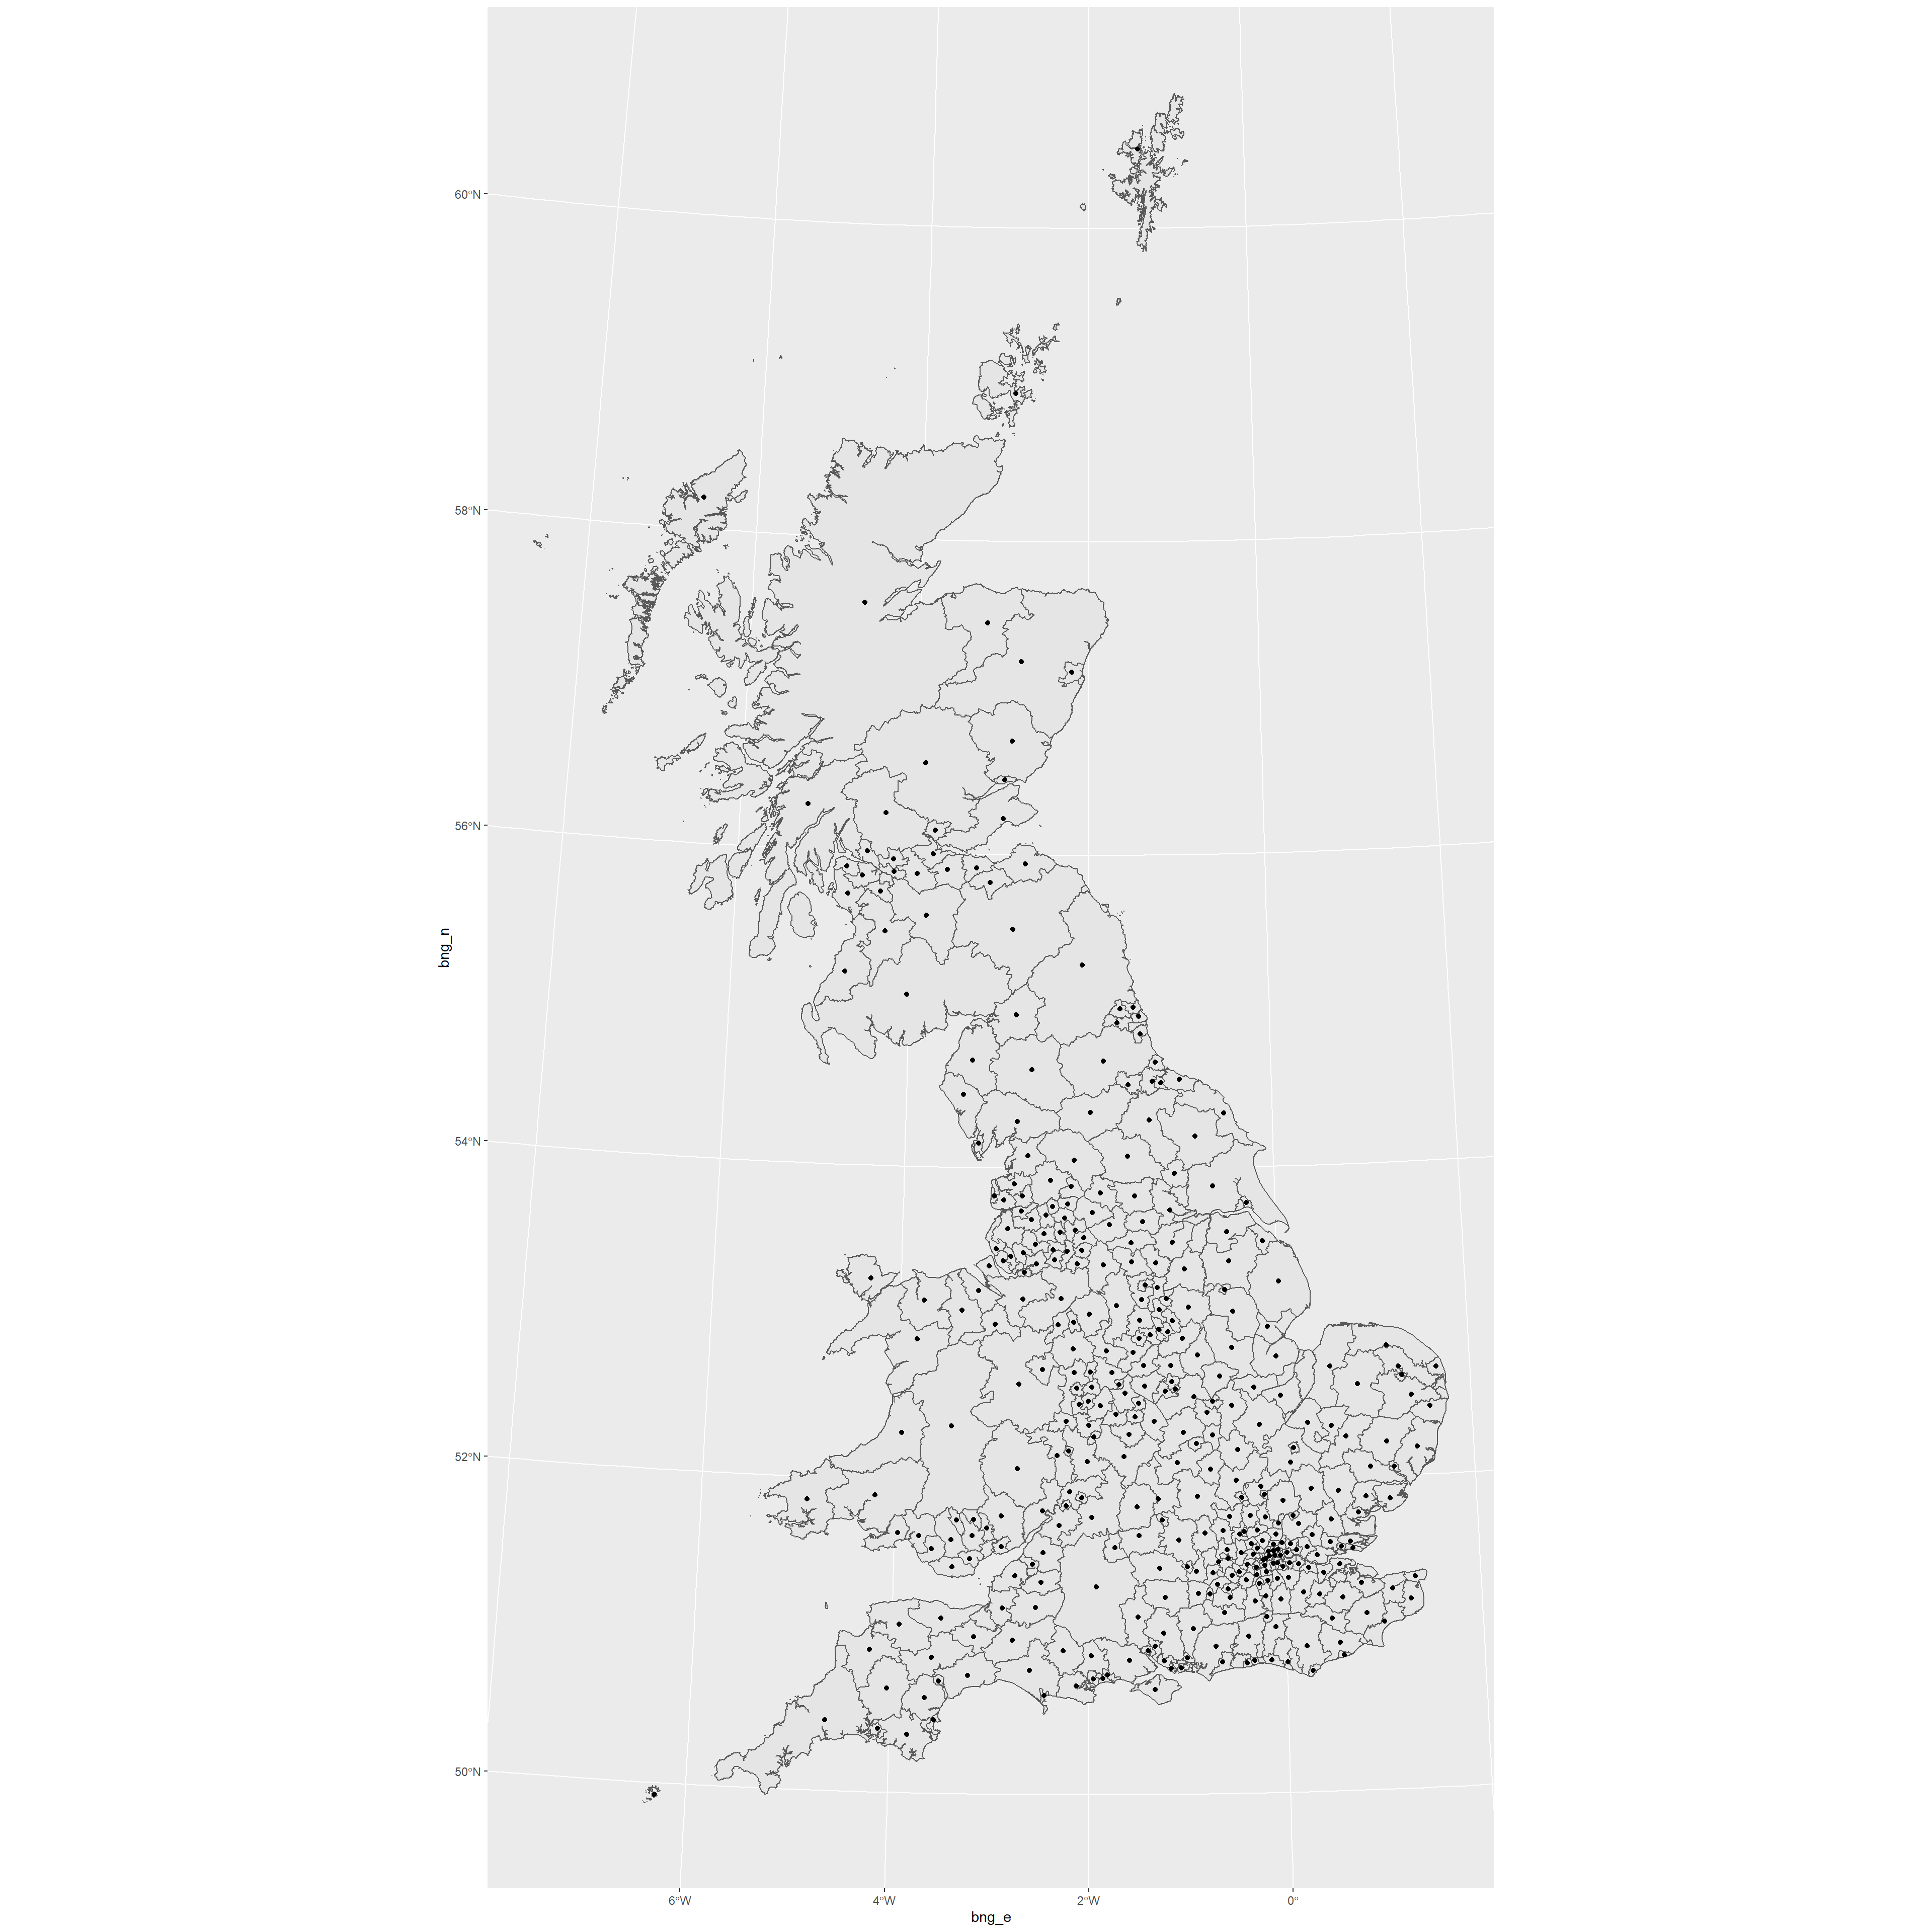
\includegraphics{pfizer_files/figure-latex/unnamed-chunk-1-1.pdf}

\begin{Shaded}
\begin{Highlighting}[]
\NormalTok{day0 =}\StringTok{ }\KeywordTok{filter}\NormalTok{(data, Day}\OperatorTok{==}\DecValTok{0}\NormalTok{)}
\NormalTok{day10 =}\StringTok{ }\KeywordTok{filter}\NormalTok{(data, Day}\OperatorTok{==}\DecValTok{10}\NormalTok{)}
\NormalTok{day22 =}\StringTok{ }\KeywordTok{filter}\NormalTok{(data, Day}\OperatorTok{==}\DecValTok{22}\NormalTok{)}


\NormalTok{day22vsday0 =}\StringTok{ }\KeywordTok{inner_join}\NormalTok{(day22,day0,}\DataTypeTok{by=}\StringTok{"condition"}\NormalTok{) }\OperatorTok\StringTok{ }\KeywordTok{mutate}\NormalTok{(}\DataTypeTok{diff=}\NormalTok{CumulativeIncidence.x}\OperatorTok{-}\NormalTok{CumulativeIncidence.y) }\OperatorTok\StringTok{ }\KeywordTok{summarise}\NormalTok{(}
  \DataTypeTok{efficacy=}\NormalTok{( }\KeywordTok{max}\NormalTok{(diff) }\OperatorTok{-}\StringTok{ }\KeywordTok{min}\NormalTok{(diff))}\OperatorTok{/}\KeywordTok{max}\NormalTok{(diff))}
\NormalTok{day22vsday0}
\end{Highlighting}
\end{Shaded}

\begin{verbatim}
## # A tibble: 1 x 1
##   efficacy
##      <dbl>
## 1    0.486
\end{verbatim}

\begin{Shaded}
\begin{Highlighting}[]
\NormalTok{day22vsday10 =}\StringTok{ }\KeywordTok{inner_join}\NormalTok{(day22,day10,}\DataTypeTok{by=}\StringTok{"condition"}\NormalTok{) }\OperatorTok\StringTok{ }\KeywordTok{mutate}\NormalTok{(}\DataTypeTok{diff=}\NormalTok{CumulativeIncidence.x}\OperatorTok{-}\NormalTok{CumulativeIncidence.y) }\OperatorTok\StringTok{ }\KeywordTok{summarise}\NormalTok{(}
  \DataTypeTok{efficacy=}\NormalTok{( }\KeywordTok{max}\NormalTok{(diff) }\OperatorTok{-}\StringTok{ }\KeywordTok{min}\NormalTok{(diff))}\OperatorTok{/}\KeywordTok{max}\NormalTok{(diff))}
\NormalTok{day22vsday10}
\end{Highlighting}
\end{Shaded}

\begin{verbatim}
## # A tibble: 1 x 1
##   efficacy
##      <dbl>
## 1    0.856
\end{verbatim}

\begin{Shaded}
\begin{Highlighting}[]
\NormalTok{day10vsday0 =}\StringTok{ }\KeywordTok{inner_join}\NormalTok{(day10,day0,}\DataTypeTok{by=}\StringTok{"condition"}\NormalTok{)}\OperatorTok\StringTok{ }\KeywordTok{mutate}\NormalTok{(}\DataTypeTok{diff=}\NormalTok{CumulativeIncidence.x}\OperatorTok{-}\NormalTok{CumulativeIncidence.y) }\OperatorTok\StringTok{ }\KeywordTok{summarise}\NormalTok{(}
  \DataTypeTok{efficacy=}\NormalTok{( }\KeywordTok{max}\NormalTok{(diff) }\OperatorTok{-}\StringTok{ }\KeywordTok{min}\NormalTok{(diff))}\OperatorTok{/}\KeywordTok{max}\NormalTok{(diff))}

\NormalTok{day10vsday0}
\end{Highlighting}
\end{Shaded}

\begin{verbatim}
## # A tibble: 1 x 1
##   efficacy
##      <dbl>
## 1    0.106
\end{verbatim}

\end{document}
